\documentclass[12pt,onecolumn,a4paper,fleqn]{article}
\usepackage[top=1in, bottom=1in, left=0.75in, right=0.75in]{geometry}
\usepackage{epsfig,graphicx,subfigure,amsthm,amsmath}
\usepackage[table,xcdraw,svgnames]{xcolor}
\usepackage{setspace}
\usepackage{mathtools}
\usepackage{fancyhdr}
\usepackage{sidecap}
\usepackage{tikz}
\usepackage{pgfplots}
\usetikzlibrary{decorations.pathreplacing}
\usepackage{relsize}
\usepackage{color,xcolor}
\usepackage[framed,numbered]{matlab-prettifier}
\usepackage{float}
\usepackage{enumerate}
\usepackage{booktabs}
\usepackage{setspace}
\usepackage{datetime}
\usepackage{xepersian}


\settextfont[Path=fonts/,BoldFont={ZarBd.ttf},BoldFeatures={Scale=0.9}]{BZar.ttf}

%\DeclarePairedDelimiter\ceil{\lceil}{\rceil}
%\DeclarePairedDelimiter\floor{\lfloor}{\rfloor}

%\definecolor{vgreen}{RGB}{104,180,104}
%\definecolor{vblue}{RGB}{49,49,255}
%\definecolor{vorange}{RGB}{255,143,102}


% title page template
\newcommand{\heading}[1]
{
	\begin{center}
		\begin{huge}
			\textbf{
				به نام خدا\\
			}
		\end{huge}
		
		\vspace*{1.5cm}
		
\includegraphics[scale=0.9]{source/sharif_logo.png}\\
		\vspace*{0.5cm}
		\begin{Large}
			\textbf{
				دانشگاه صنعتی شریف\\
				\vspace*{0.25cm}
				دانشکده مهندسی کامپیوتر\\
			}
		\end{Large}
		\vspace*{3cm}
		\begin{huge}
			\textbf{
				آزمایشگاه معماری کامپیوتر\\
				\vspace*{0.75cm}
			}
		\end{huge}
		
		\begin{Large}
			\textbf{
				آزمایش هفتم:\\
				#1\\
			}
		\end{Large}
		
		\noindent\rule[1ex]{\linewidth}{1pt}\\
		\vspace*{0.5cm}
		\begin{table}[H]
			\centering
			\begin{tabular}{|c|c|}
				\hline
				\multicolumn{2}{|c|}{\textbf{اطلاعات تیم}}
				\\ \hline
				\textbf{نام اعضا} & \textbf{شماره دانشجویی}
				\\ \hline
				متین داغیانی & 98106456
				\\ \hline
				بردیا محمدی & 98171104
				\\ \hline
				محمدجواد هزاره & 98101074
				\\ \hline 
			\end{tabular}
		\end{table}
		\begin{Large}				
			\vspace*{0.75cm}
			\textbf{
				زمستان 1400
			}
		\end{Large}			
	\end{center}
}

\pagestyle{fancy}
\fancyhf{}
\rhead{\textbf{آزمایشگاه معماری کامپیوتر}}
%%--------------------[should change]---------------------
\chead{\textbf{گزارش آزمایش هفتم}}
%%--------------------[should change]---------------------
\lhead{\textbf{\nouppercase{\rightmark}}}
\cfoot{({\thepage})}
\renewcommand{\headrulewidth}{1pt}
\renewcommand{\footrulewidth}{1pt}
\renewcommand{\sectionmark}[1]{\markright{#1}}
\renewcommand{\subsectionmark}[1]{\markright{#1}}
%\newdateformat{monthyeardate}{%
%	\monthname[\THEMONTH], \THEYEAR}

\onehalfspacing
\begin{document}
	%%% title pages
	\large
	\begin{titlepage}
		\heading{استفاده از حافظه داده و دستورات پرش}
		\thispagestyle{empty}
	\end{titlepage}	
	\pagebreak
	
	%%% contents page
	\tableofcontents
	\thispagestyle{empty}
	\pagebreak
	
	%%% main document
	\section{هدف آزمایش}
	در این آزمایش قصد داریم تا با اضافه کردن امکانات متعدد مدار طراحی شده در آزمایش شماره شش را تکمیل کرده و در نهایت به یک کامپیوتر ساده با معماری \lr{Harvard}دست یابیم. به همین جهت در گام اول یک \lr{RAM} با گنحایش 32 بایت را به مدار اضافه می کنیم و در نتیجه امکان ذخیره مقادیر بینابینی را در پیدا خواهیم کرد. هم چنین در ادامه امکان استفاده از دستورات پرش شرطی و غیر شرطی را فراهم خواهیم کرد. در شکل زیر دیاگرام بلوکی مدار  نهایی را مشاهده می کنید:
	\begin{figure}[H]
				\centering
				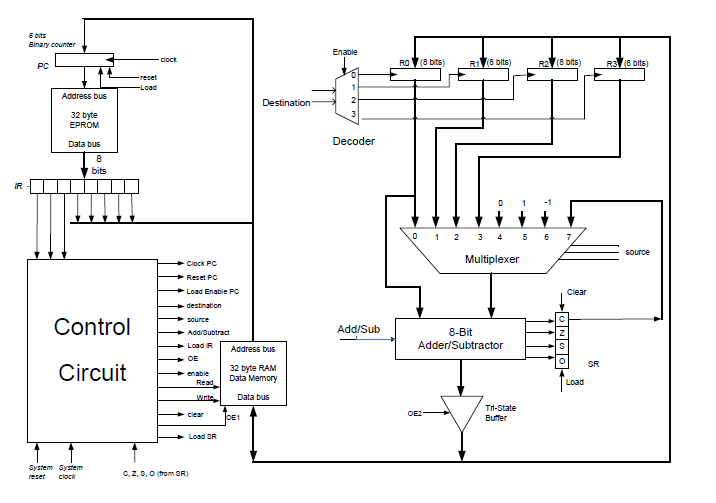
\includegraphics[width=0.68\textwidth]{source/1.png}
				\caption{بلوک دیاگرام سیسیتم}
				\label{fig:1}
	\end{figure}
	
	همان طور که در شکل مشخص است، یک حافظه داده با ظرفیت 32 بایت اضافه شده است که امکان ذخیره و بازیابی داده ها را فراهم می کند. این حافظه از طریق سیگنال های کنترلی \lr{Read} و \lr{Write} با واحد کنترل در ارتباط است و هم چنین به کمک خطوط ارتباطی موچود به \lr{PC} نیز دسترسی دارد. هم چنین در قسمت جریان داده رجیسترهای \lr{flag} اضافه شده اند که برای دستورات پرش شرطی مورد ارزیابی قرار می گیرند.
	
نمای کلی مدار پیاده سازی شده در ادامه آمده است.
	\begin{figure}[H]
					\centering
					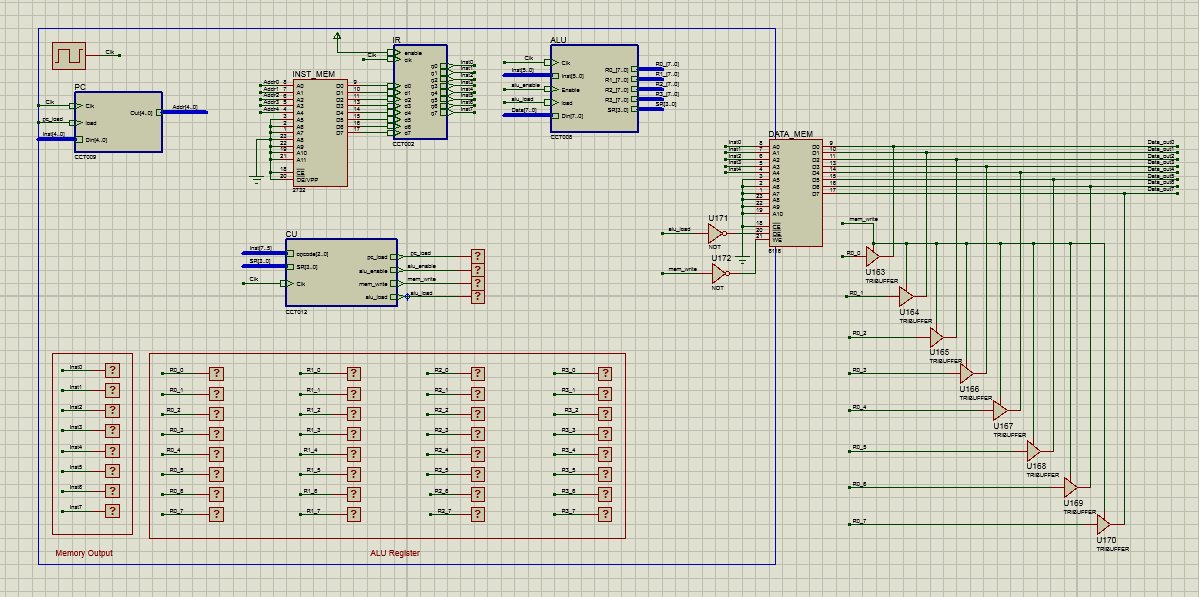
\includegraphics[width=0.68\textwidth]{source/2.png}
					\caption{نمای کلی سیستم پیاده سازی شده}
					\label{fig:2}
	\end{figure}


	\section{مراحل طراحی و پیاده‌سازی مدار}
	\subsection {ماژول‌های مورد نیاز و شروع به کار مدار}
	همانطور که در شکل 1 مشخص است، برای کنترل سیگنال های کنترلی به واحد \lr{CU} نیاز داریم. به علاوه با توجه به اضافه شدن دستورات پرش شرطی و غیر شرطی ماژول \lr{PC} نسبت به آزمایش قبلی به روز شده است. هم چنین ماژول دیگری به نام \lr{DATAMEM} نیز برای ذخیره و بازیابی داده ها در نظر گرفته شده است. در ادامه به بررسی دقیق تر هر ماژول خواهیم پرداخت.
	
		\subsection{ماژول \lr{PC}}
			\begin{figure}[H]
						\centering
						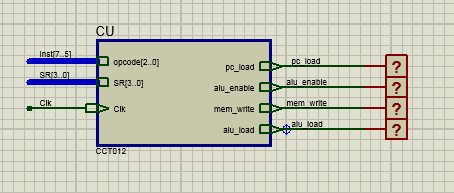
\includegraphics[width=0.68\textwidth]{source/3.png}
						\caption{ماژول \lr{PC}}
						\label{fig:3}
		\end{figure}
		
		برای پیاده سازی این ماژول از یک شمارنده بالا/پایین دودویی استفاده شده است که امکان لود موازی را نیز دارد. (تراشه شماره 4516). همان طور که در تصویر زیر مشخص است، خطوط 5 بیتی داده های ورودی به ورودیهای تراشه متصله است که در هنگام اجرای دستور پرش به کمک سیگنال کنترلی \lr{load} در تراشه بار می شود. 
	
	\section{تست مدار}
\end{document}